\section{Overview}
\label{sec:ktoctou-overview}




\subsection{Threat Model}
\label{sec:ktoctou-threatmodel}

Kernel TOCTOU is a local privilege escalation vulnerability. The vulnerability could allow local users or malicious software to gain full root privileges. We assume that an attacker has a user account that can upload and run arbitrary programs with user privilege or access such a program. The attacker has arbitrary memory reads and writes primitives. He is also able to call any system service or load any library. The DEP policy (\textbf{W}rite $\oplus$ e\textbf{X}ecute) and ASLR is not necessary. We assume the attacker has full knowledge about the system kernel, including the memory layout. However, he can not read or write any kernel memory because a classical operating system would not allow it. The attacker aims at running arbitrary code in the kernel, hence obtains the highest privilege.

We endeavor at the Windows OS, a complicated operating system. Linux kernel is out of scope. %because it already utilizes the Intel processor feature SMAP conventionally (\autoref{sec:ktoctou-background}).
Considering we leverage a hardware feature from the Intel processor, The host system needs to have an Intel processor with SMAP capability.

\subsection{High-Level Design and Challenges}

The kernel double fetching a user address may cause a TOCTOU vulnerability. There are two ways to prevent exploitation; one is to drop the kernel's double-fetch action; the other is to prevent data mismatch between fetches. From a practical point of view, we can not decline the kernel's double-fetch behavior. Therefore, this paper proposes a framework to prevent data mismatch between fetches. The high-level idea is that when the kernel accesses a user address, we freeze the containing page so that no other user thread can overwrite it.

However, there have been many challenges here:

\begin{itemize}
	\item How can we know when the kernel accesses a user address?
	\item It is overkill to freeze an entire page just for one variable and reads should allow.
	\item The two fetches should happen within a short time, more specifically, within the same system call.
	\item Windows is a complex operating system. How can we practically enable a system-wide hardware feature such as SMAP without crashing the system?
\end{itemize}



\subsection{Approach Overview}


How to get notified when the kernel accesses a user address is the biggest challenge. Since the processor reading memory is such an ordinary operation, no official hardware feature is available for monitoring it in a broad range of memory. To solve this challenge, we abuse a hardware feature SMAP.  Originally, SWAP is designed to prevent the attacker from tricking the kernel into getting shellcode or malicious data from userspace. However, one unique characteristic of this feature is that when the kernel accesses a user address, the processor raises a page fault exception. This feature accurately serves our purpose so that we will leverage it in a novel way to solve the challenge.

Subject to the x86 architecture, the protection has to base on the page granularity. To protect even one byte, we have to protect an entire page.
First, we separate the subsequent user reads from writes because the reads are harmless.  When we temporarily release a page, we set this page as read-only to ensure no writing. When a user writes on the protected page, we make the thread suspend on the writing instruction until the current system call ends.

As previously mentioned in ~\autoref{sec:ktoctou-background}, the kernel-level TOCTOU vulnerabilities happen inside individual system calls. We hook Windows internal functions to know when a system call ends and releases the pages it accessed. Also, we monitor the creation and termination for both processes and threads and use Windows internal data structures to distinguish each thread.

We develop a light-weight hypervisor to confine the SMAP feature into specific processes. It makes debugging less painful to us, and it is also necessary to prevent nested SMAP exceptions that cause a dead loop.

~\autoref{fig:ktoctou-overview} shows the high-level overview. The hypervisor enables SMAP only in one process, which is the one currently running on the processor. The kernel has accessed three user pages, as marked in the user process memory space, and one user thread in the same process tries to access those pages. Notice the read is allowed. The protected page is temporarily released and set read-only. However, the write is not permitted for the moment; the page fault handler suspends the thread to avoid causing any data inconsistency in the kernel.

\begin{figure}[th]
  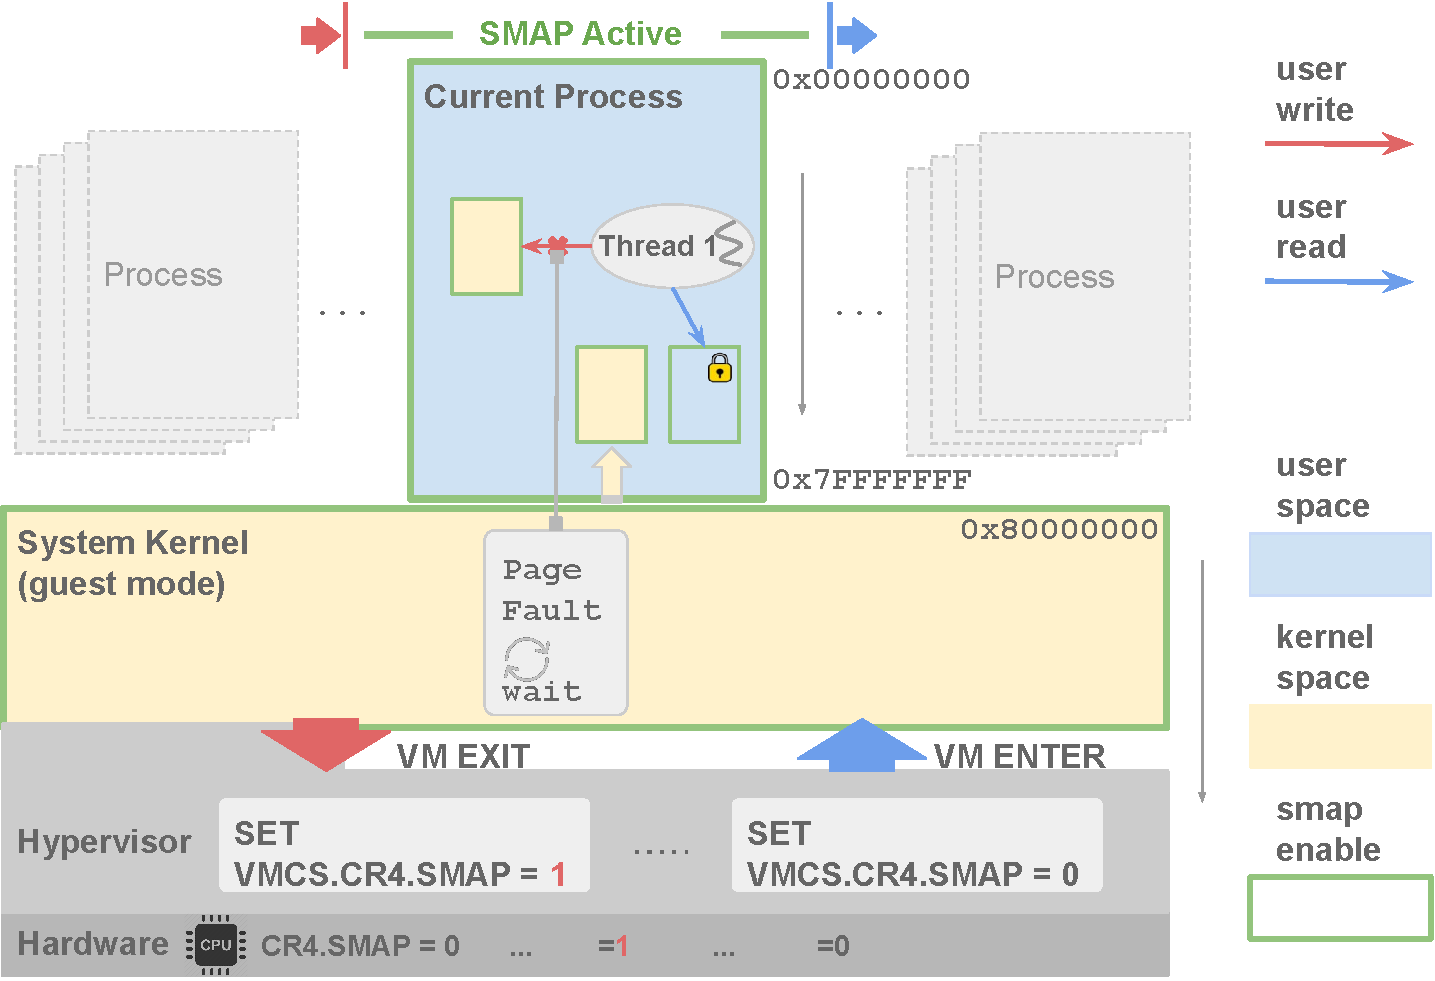
\includegraphics[width=0.47\textwidth]{figures/ktoctou-overview2}
  \centering
  \caption{The hypervisor is capable of confining the system-wide feature SMAP into one process. When the hypervisor catches the process context switch events, it changes the SMAP enable bit in the CR4 register to only set during the target process. The processor raises page fault exception when the kernel accesses userspace so that we can protect those pages. Thread 1 can read a protected page but can not write. The read is allowed by automatically setting the protected page back to userspace with a read-only permit. However, when the write instruction raises an exception, the page fault handler suspends the thread until the system call ends.}
  \label{fig:ktoctou-overview}
\end{figure}
